\chapter{System Architecture and Design}\label{ch:design}

\section{Overall System Architecture}
The system is built as three tiers that communicate only with the tier next to them
(Figure~\ref{fig:arch}).

\fig{arch_system.png}{Overall architecture: presentation, application and data tiers}{fig:arch}{0.5}

\begin{description}
\item[Tier 1, presentation.] A Spring Boot application (port 8080) that renders HTML on
the server with Thymeleaf and styles it with Tailwind CSS. It has 18 MVC controllers and
70 templates. It never touches the database. It calls the backend through one thin client
class, \cd{ApiClient}, and keeps the user's tokens and permissions in a server-side
session, so the tokens never reach browser JavaScript.
\item[Tier 2, application.] A Spring Boot REST service (port 8000). Every request passes
a JWT filter, then a permission interceptor, then a controller, a service that runs the
business rules inside a transaction, and a small data-access helper. It exposes 225
operations on 151 paths and publishes its contract with Swagger UI at \cd{/docs}.
\item[Tier 3, data.] A MySQL 8.0 database with 63 tables, 6 views, 5 triggers, 3 stored
procedures and 25 additional indexes, using the InnoDB engine and the \texttt{utf8mb4}
character set.
\end{description}
Two side services complete the picture. Notifications are handed to a provider interface
(a mock in this build), and uploaded documents are stored on the local file system with
only their path in the database.

The request path through the application tier is detailed in Figure~\ref{fig:request}.
Two points deserve emphasis. Authorisation happens \emph{before} any controller code, so a
forgotten check in a controller cannot expose data. And notifications are queued during the
transaction but delivered only \emph{after} it commits, so a rolled-back action never
sends a message.

\fig{flow_request.png}{Life cycle of one backend request, from token check to response}{fig:request}{0.88}

\section{Component and Module Description}
\subsection{Backend packages}
Table~\ref{tab:packages} shows how the backend source is organised. The main source has
about 11\,300 lines of Java and the test source about 4\,400 lines.

\begin{table}[H]
\centering\small
\caption{Backend packages and their responsibilities}\label{tab:packages}
\begin{tabularx}{\linewidth}{@{}p{2.2cm}X@{}}
\toprule \textbf{Package} & \textbf{Responsibility}\\ \midrule
\cd{web} & REST controllers (16 files). Each method is annotated with \cd{@Public}, \cd{@Requires} or \cd{@RequiresAny}; the nine reference-data resources are generated from one base class\\
\cd{dto} & Immutable request and response records with Bean Validation annotations\\
\cd{service} & Business rules, one class per area, each method running in a transaction\\
\cd{core} & Shared infrastructure: \cd{Db} (queries, row locks, paging), \cd{QB} (query builder), \cd{Audit}, \cd{Perms}, \cd{PageParams}, error mapping, current-user resolution\\
\cd{domain} & 63 JPA entities, one per table, using plain foreign-key ids\\
\cd{security} & JWT service, authentication filter, BCrypt password helper, Spring Security configuration\\
\cd{config} & JSON naming and formatting, CORS, OpenAPI\\
\cd{cli} & Start-up commands: apply the schema, bootstrap the first administrator\\
\bottomrule
\end{tabularx}
\end{table}

\subsection{Functional modules}
The business logic is divided into modules that match the schema modules
(Table~\ref{tab:modules}). Each module is a service class (or a small group of them) with
its own controller.

\begin{table}[H]
\centering\small
\caption{Functional modules, their services and the main tables they own}\label{tab:modules}
\begin{tabularx}{\linewidth}{@{}p{2.9cm}p{3.5cm}X@{}}
\toprule \textbf{Module} & \textbf{Service classes} & \textbf{Main tables}\\ \midrule
Authentication and RBAC & \cd{AuthService}, \cd{UserLoader}, \cd{RbacService} & users, roles, permissions, user\_roles, role\_permissions\\
Citizens and staff & \cd{CitizenService}, \cd{EmployeeService}, \cd{OfficeService} & persons, addresses, citizens, employees, employee\_postings, rto\_offices, counters\\
Reference data & \cd{ReferenceService} & regions, vehicle\_*, fuel\_types, licence\_classes, document\_types, service\_types, violation\_types, permit\_types\\
Applications & \cd{ApplicationService}, \cd{DocumentService}, \cd{AppointmentService} & applications, application\_status\_history, documents, appointment\_slots, appointments\\
Licensing & \cd{LicenceService} & learner\_licences, driving\_licences, licence\_class\_assignments, driving\_tests, driving\_schools\\
Vehicles & \cd{VehicleService}, \cd{OwnershipService} & vehicles, vehicle\_ownerships, ownership\_transfers\\
Compliance and permits & \cd{ComplianceService}, \cd{PermitService} & inspections, fitness, pollution, insurance, road tax, routes, permits\\
Enforcement & \cd{ViolationService} & violations, challans, challan\_violations\\
Payments & \cd{PaymentService}, \cd{Fees} & payments, payment\_attempts, refunds, fee\_structures\\
Support and oversight & \cd{SupportService}, \cd{Notifications}, \cd{DashboardService}, \cd{Audit} & complaints, appeals, notifications, audit\_logs\\
\bottomrule
\end{tabularx}
\end{table}

\subsection{Portal components}
The portal has one controller per area (applications, citizens, vehicles, licences,
permits, compliance, violations, payments, support, employees, ownership transfers,
appointment slots, authentication, dashboard) and four administration controllers (users,
roles, offices, reference data). Four small classes provide the plumbing:
\begin{itemize}
\item \cd{ApiClient} calls the backend with the session's bearer token, refreshes it once on a 401 response, turns error bodies into one exception type, and normalises paging and search parameters so that hand-edited URLs degrade gracefully.
\item \cd{UserSession} holds the tokens, the user's roles and the permission set for the current browser session.
\item \cd{WebConfig} redirects anyone who is not signed in to the login page.
\item \cd{GlobalAdvice} supplies the signed-in user to every template and converts exceptions into friendly pages with the correct HTTP status.
\end{itemize}
Shared Thymeleaf fragments (\cd{layout.html} and \cd{ui.html}) give every page the same
sidebar, form controls, pager and status badges.

\section{Architecture Selection and Justification}
\subsection{Choice}
We chose a layered client--server design with a separate, server-rendered portal. The
backend is an independent REST service; the portal is one possible client.

\subsection{Reasons}
\begin{enumerate}
\item \textbf{Separation of concerns.} Rules sit in services, access control in one interceptor, persistence in one helper. A change to an access rule does not touch a screen.
\item \textbf{A reusable API.} Because the backend is not tied to the portal, a mobile application or another office system can use the same 225 operations.
\item \textbf{Safer tokens.} In a server-rendered portal the access token stays on the server side of the browser connection; no JavaScript running in the page can read it.
\item \textbf{Fewer moving parts.} No JavaScript framework or build pipeline is needed. Tailwind is loaded from a CDN and Thymeleaf renders pages.
\item \textbf{Testability.} The backend can be tested against a real database without a browser, and the portal can be crawled over plain HTTP.
\end{enumerate}

\begin{table}[H]
\centering\small
\caption{Alternatives considered}\label{tab:alt}
\begin{tabularx}{\linewidth}{@{}p{3.6cm}XX@{}}
\toprule \textbf{Alternative} & \textbf{Advantage} & \textbf{Why not chosen}\\ \midrule
One application with controllers and views together & Fewer deployments & The API could not be reused cleanly; rules and screens would be mixed\\
Single-page application (React or similar) & Rich interaction & Needs a JavaScript toolchain; the token would live in the browser; unnecessary for form-driven office work\\
Microservices per module & Independent scaling & Distributed transactions would complicate exactly the multi-step operations we want to keep atomic\\
\textbf{Layered backend + server-rendered portal} & Clear layering, reusable API, simple tooling & Two processes must both run\\
\bottomrule
\end{tabularx}
\end{table}

\section{Data Flow Diagrams}
Figure~\ref{fig:dfd0} is the context diagram: three groups of people and one external
service interact with a single process. Figure~\ref{fig:dfd1} decomposes it into seven
processes and eight data stores. Figure~\ref{fig:dfd2} decomposes process 2.0 (citizen
and application management), the busiest one.

\fig{dfd0.png}{Data flow diagram, level 0 (context)}{fig:dfd0}{0.3}
\fig{dfd1.png}{Data flow diagram, level 1}{fig:dfd1}{0.5}
\fig{dfd2.png}{Data flow diagram, level 2 for process 2.0}{fig:dfd2}{0.5}

\section{UML Diagrams}
\subsection{Use case diagrams}
The use cases are split into three diagrams by actor group: citizens and counter
clerks (left of Figure~\ref{fig:uc1}), officers and inspectors (right of
Figure~\ref{fig:uc1}), and enforcement, accounts and administration
(Figure~\ref{fig:uc3}).

\begin{figure}[H]
\centering
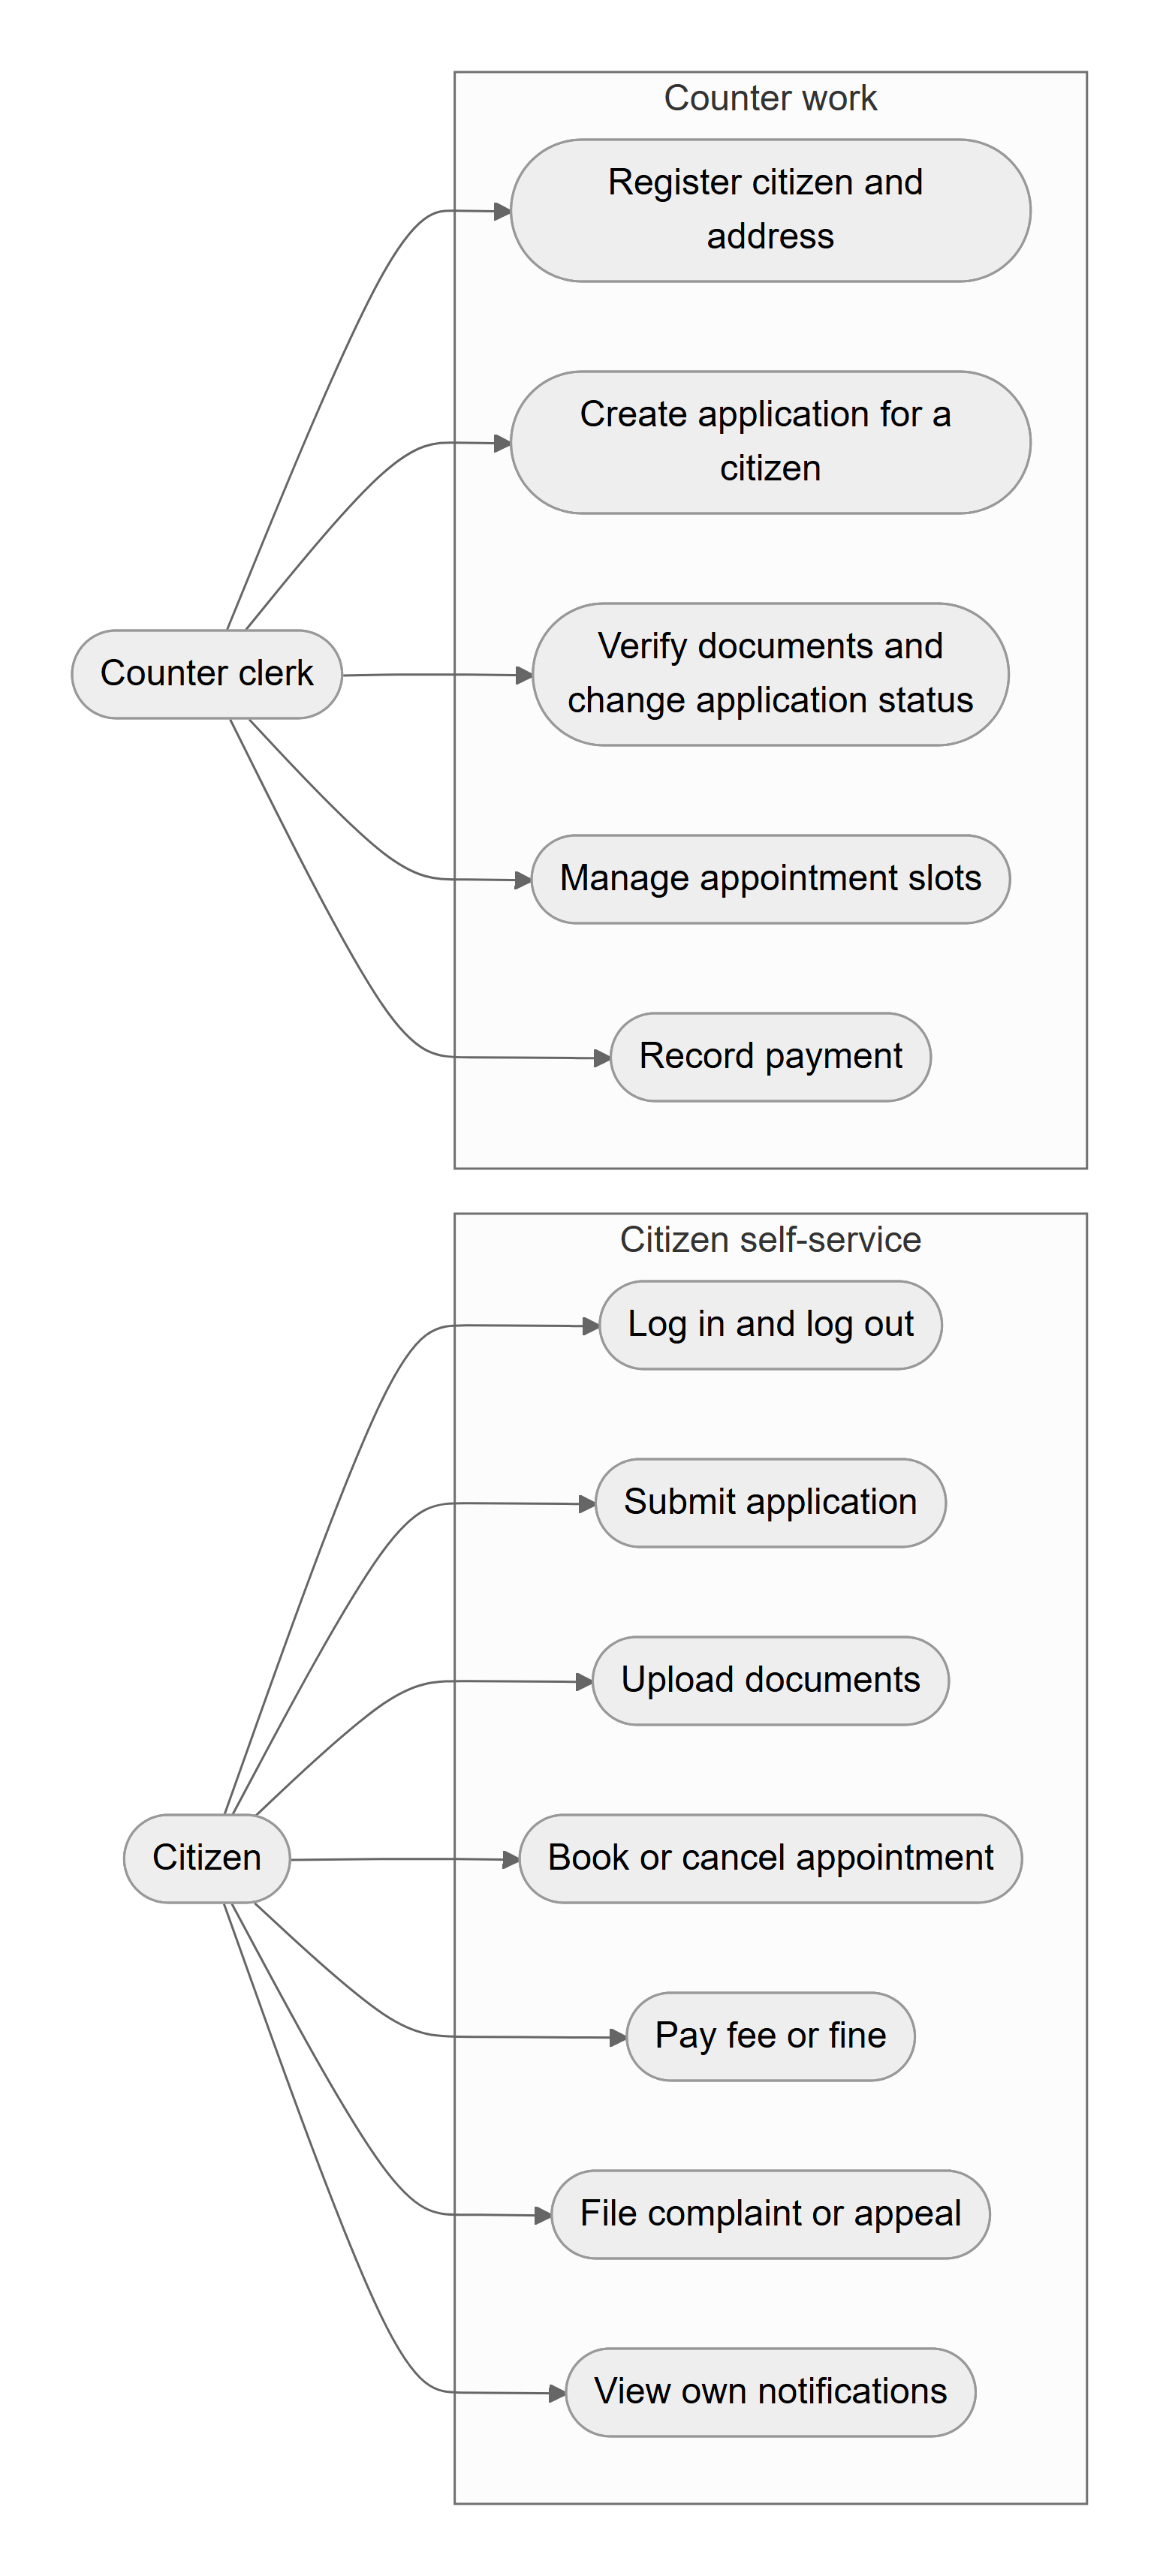
\includegraphics[height=0.42\textheight,keepaspectratio]{usecase_citizen.png}\hfill
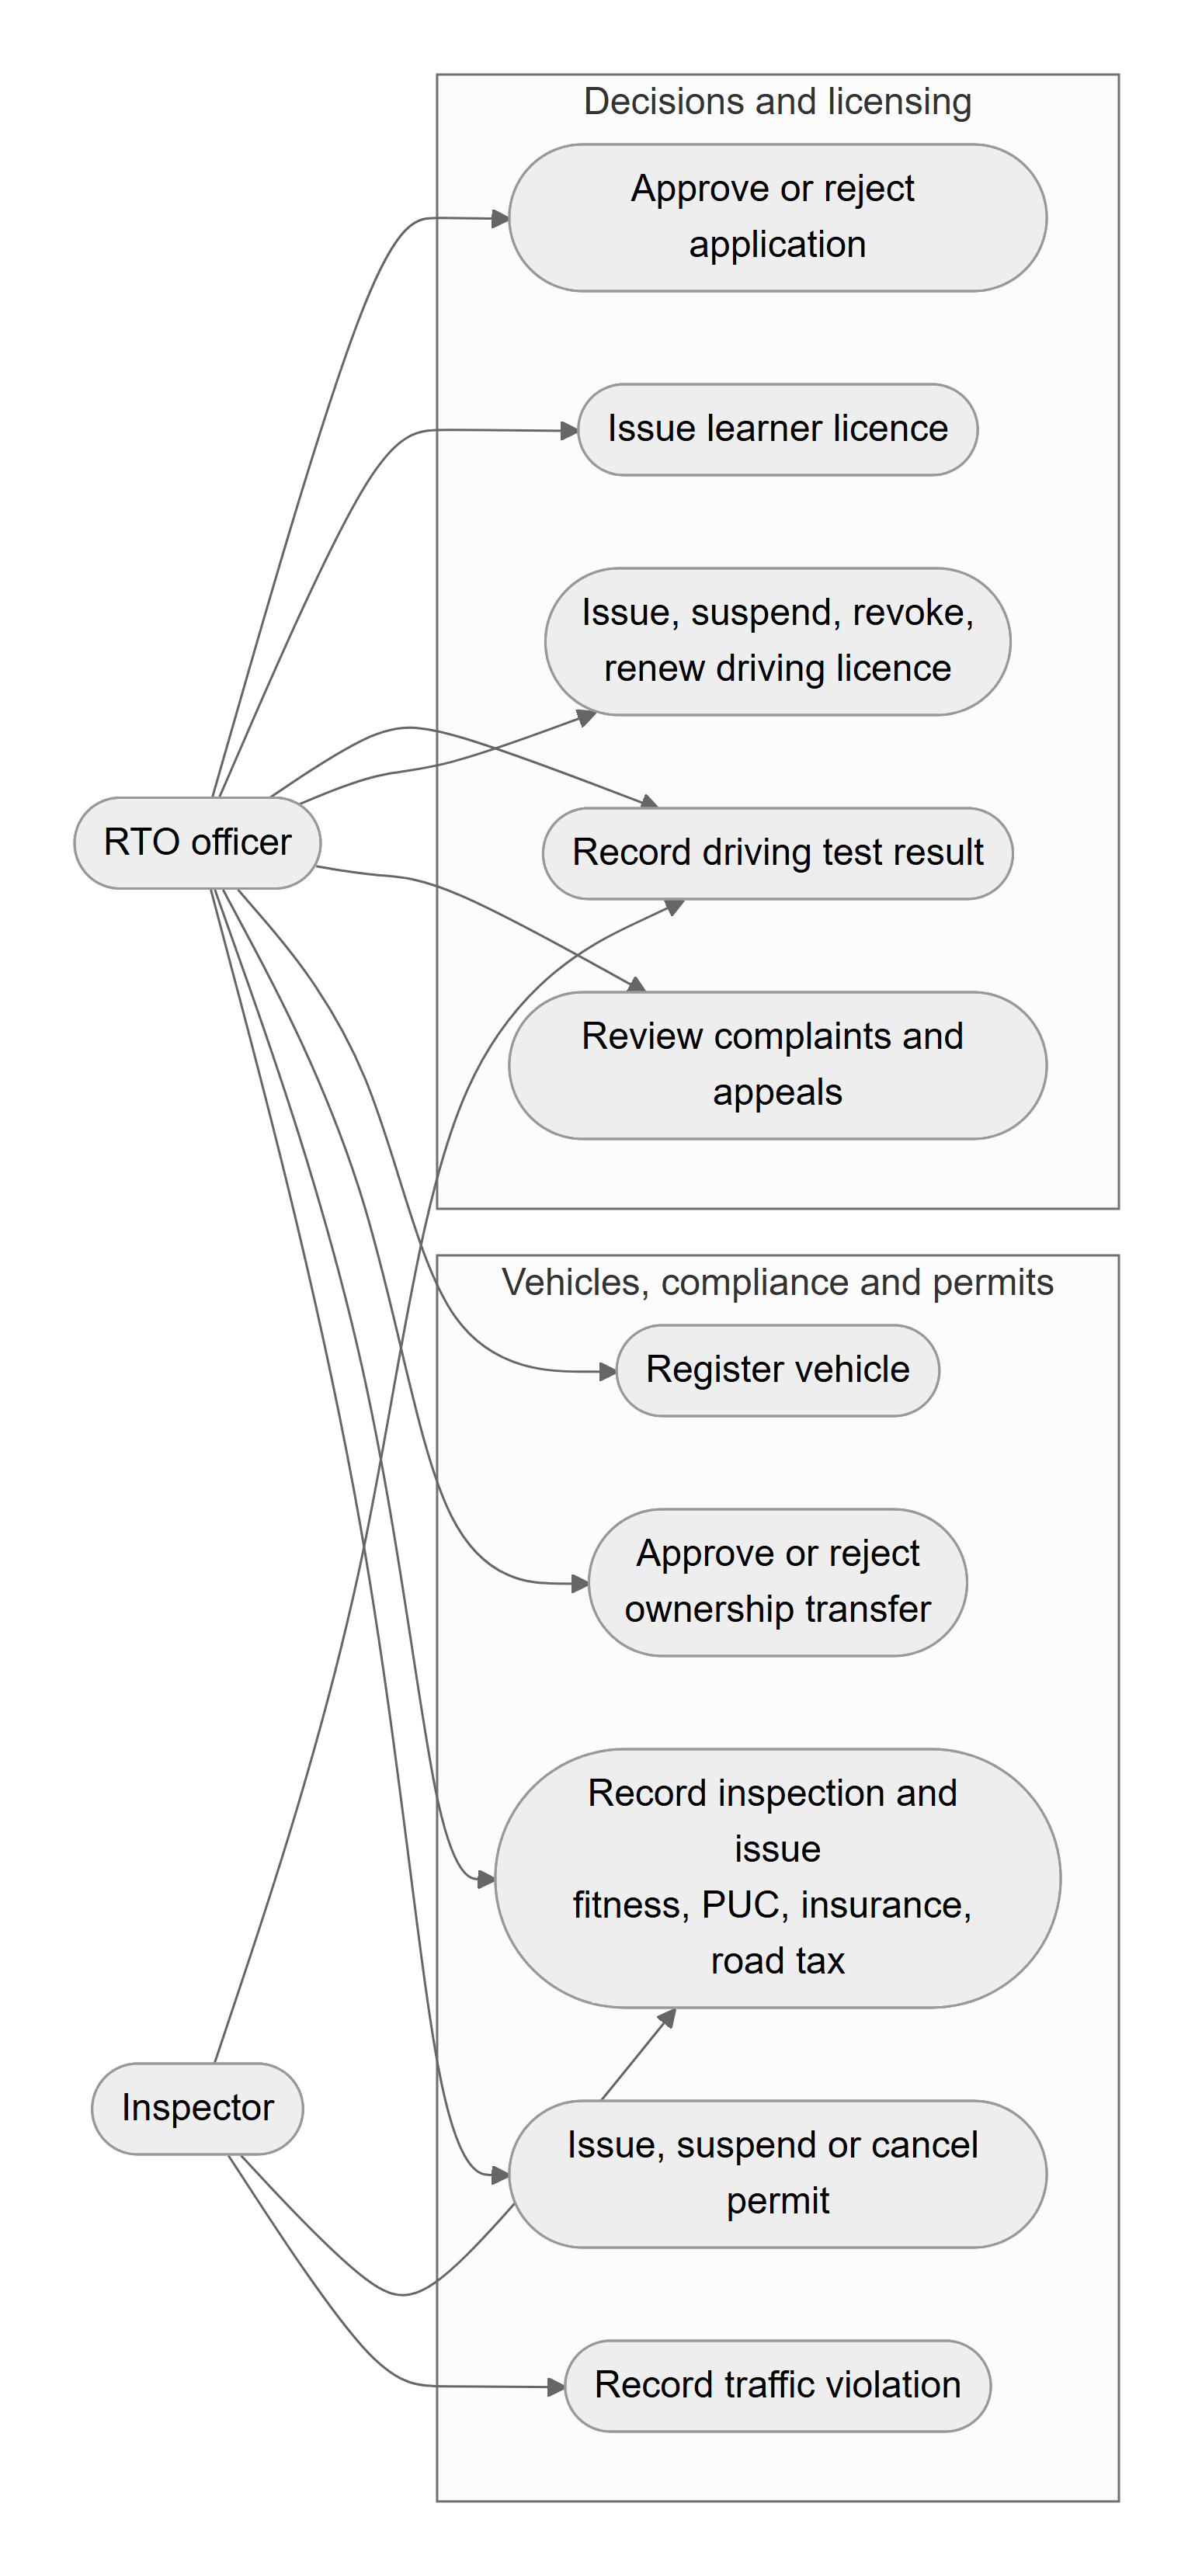
\includegraphics[height=0.42\textheight,keepaspectratio]{usecase_officer.png}
\caption{Use case diagrams: (left) citizen and counter clerk, (right) RTO officer and inspector}\label{fig:uc1}
\end{figure}
\begin{figure}[H]
\centering
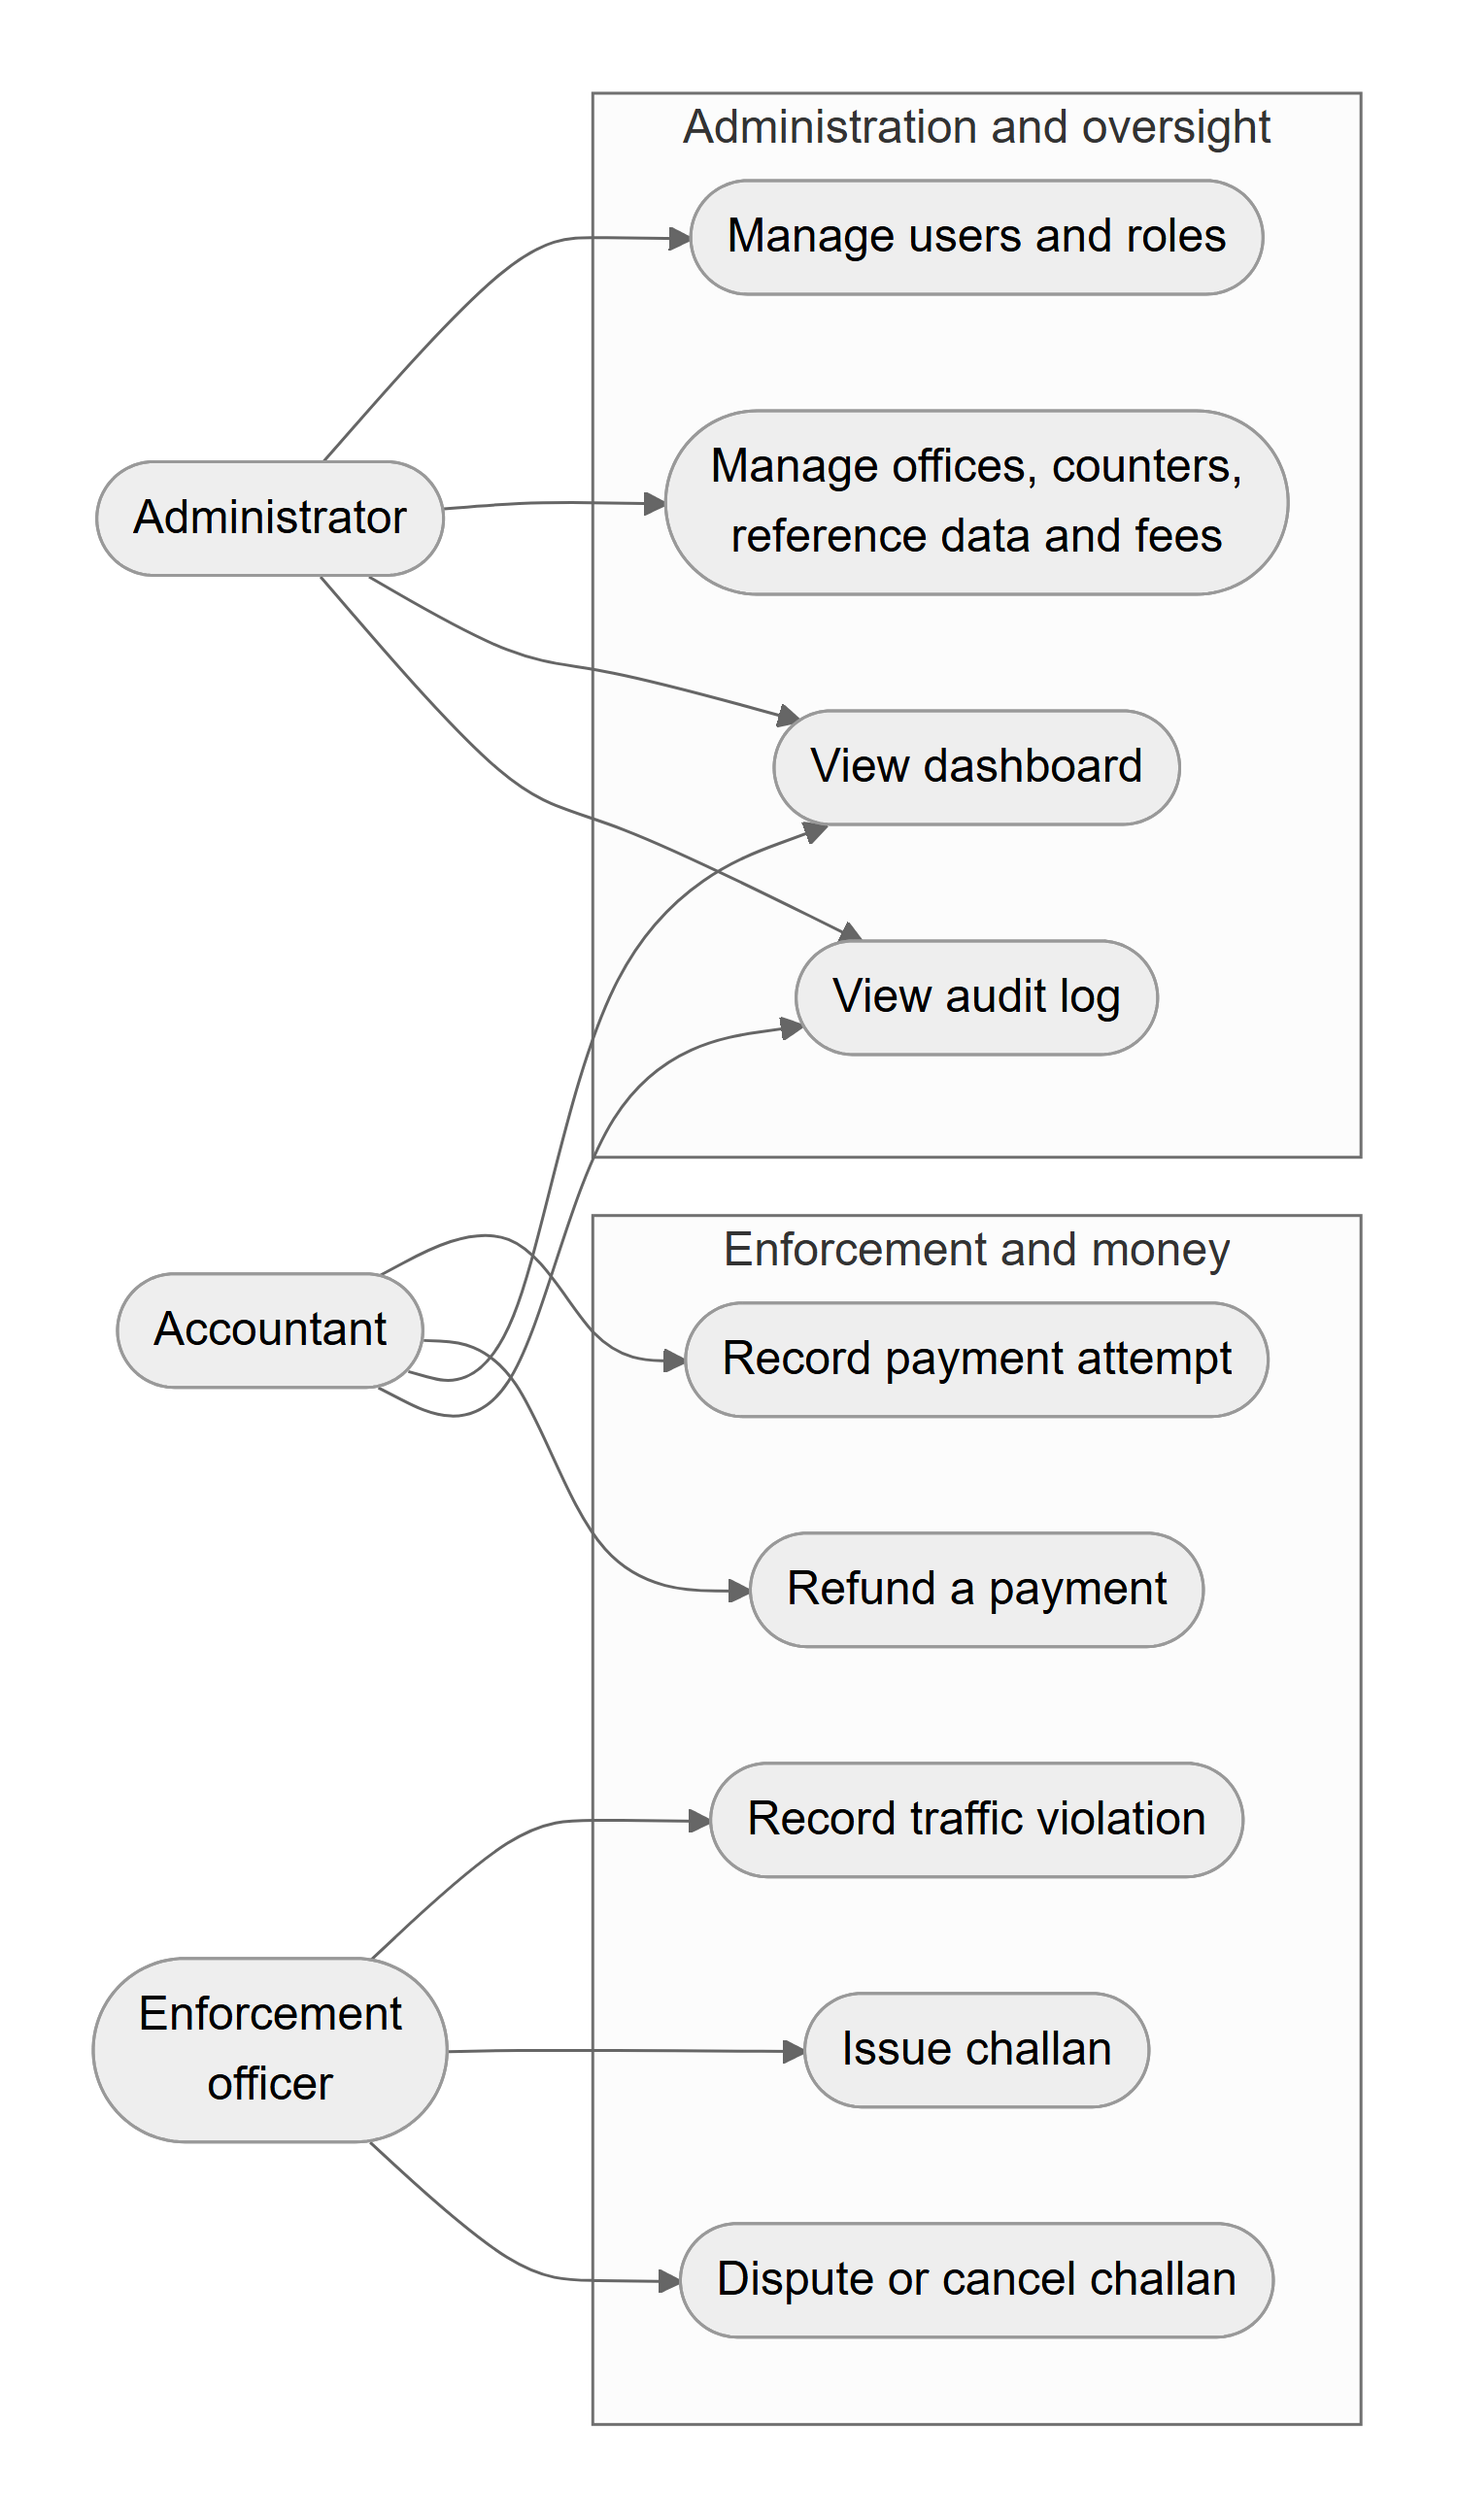
\includegraphics[height=0.40\textheight,keepaspectratio]{usecase_admin.png}
\caption{Use case diagram: enforcement officer, accountant and administrator}\label{fig:uc3}
\end{figure}

\subsection{Class diagram}
Figure~\ref{fig:class} shows the core classes and how they depend on each other. The
important design points are that services depend on \cd{Db}, \cd{Audit} and
\cd{Notifications} but never on each other's data access, and that
\cd{Notifications} depends on the \cd{NotificationProvider} interface, whose mock
implementation can be replaced without changing any caller.

\fig{class_core.png}{Class diagram of the core services and infrastructure}{fig:class}{0.62}

\subsection{Sequence diagrams}
Figure~\ref{fig:seqlogin} shows sign-in and Figure~\ref{fig:seqtransfer} shows approval
of an ownership transfer, the most delicate transaction in the system.

\fig{seq_login.png}{Sequence diagram: sign-in and permission loading}{fig:seqlogin}{0.5}
\fig{seq_transfer.png}{Sequence diagram: approval of an ownership transfer in one transaction}{fig:seqtransfer}{0.4}

\subsection{Activity diagram}
Figure~\ref{fig:activity} follows one service application from creation to completion,
including the loops for missing or rejected documents.

\fig{activity_app.png}{Activity diagram of the application life cycle}{fig:activity}{0.82}

\subsection{State machine diagrams}
Every status field that matters has a transition table in the service code; anything not
in the table is refused with a 409 response. Figure~\ref{fig:stateapp} shows the
application workflow and Figure~\ref{fig:stateother} shows the licence, challan, permit
and vehicle machines.

\fig{state_application.png}{State machine of an application (nine states)}{fig:stateapp}{0.45}
\fig{state_others.png}{State machines of driving licence, challan, permit and vehicle}{fig:stateother}{0.4}

\subsection{Component and deployment diagram}
Figure~\ref{fig:deploy} shows the processes and ports of the development deployment.
Everything runs on one machine; the backend and portal are separate JVM processes.

\fig{deploy.png}{Component and deployment view of the development setup}{fig:deploy}{0.3}

\section{Database Design}
\subsection{Overview}
The schema is created by thirteen scripts, one per module, run in dependency order
(Table~\ref{tab:dbmodules}). The order is not arbitrary: it is a topological order of the
foreign-key graph. We checked this mechanically. Across all 91 foreign keys, no table is
created before a table it references; the longest chain of dependencies has depth six,
and the only self-reference is \cd{regions.parent_region_id}, which lets regions form a
tree.

\begin{table}[H]
\centering\small
\caption{Schema modules, creation scripts and table counts}\label{tab:dbmodules}
\begin{tabularx}{\linewidth}{@{}p{0.9cm}p{3.2cm}cX@{}}
\toprule \textbf{File} & \textbf{Module} & \textbf{Tables} & \textbf{Tables created}\\ \midrule
02 & Reference data & 11 & regions, vehicle\_manufacturers, vehicle\_models, vehicle\_types, fuel\_types, licence\_classes, document\_types, service\_types, violation\_types, permit\_types, payable\_types\\
03 & Identity & 3 & persons, addresses, citizens\\
04 & Office structure & 4 & rto\_offices, departments, designations, counters\\
05 & Employees & 2 & employees, employee\_postings\\
06 & Access control & 5 & users, roles, permissions, user\_roles, role\_permissions\\
07 & Applications & 6 & applicants, applications, application\_status\_history, documents, appointment\_slots, appointments\\
08 & Licensing & 8 & driving\_schools, driving\_instructors, test\_centres, learner\_licences, driving\_licences, licence\_class\_assignments, licence\_status\_history, driving\_tests\\
09 & Vehicles & 3 & vehicles, vehicle\_ownerships, ownership\_transfers\\
10 & Compliance & 5 & vehicle\_inspections, fitness\_certificates, pollution\_certificates, insurance\_policies, road\_tax\_records\\
11 & Permits & 4 & routes, route\_segments, permits, permit\_status\_history\\
12 & Violations & 4 & violations, challans, challan\_violations, challan\_status\_history\\
13 & Payments & 4 & fee\_structures, payments, payment\_attempts, refunds\\
14 & Support & 4 & notifications, complaints, appeals, audit\_logs\\
\midrule
 & \textbf{Total} & \textbf{63} & \\
\bottomrule
\end{tabularx}
\end{table}

\subsection{Entity--relationship diagrams}
The twelve diagrams that follow cover all 63 tables. They were generated from the live
database, so the keys and relationships shown are the real ones. In each diagram
\texttt{PK} marks a primary key, \texttt{FK} a foreign key and \texttt{UK} a unique key.
A solid line with a single bar means the referencing column is mandatory; a line with a
circle means it may be empty. Tables from other modules appear as small boxes with only
their primary key.

\fig{er_org.png}{ER diagram: organisation and staff}{fig:er1}{0.45}
Offices belong to regions (a tree through \cd{parent_region_id}); counters belong to an
office; an employee has a designation and any number of dated postings to an office and a
department. A generated column guarantees that an employee has at most one open posting.

\fig{er_identity.png}{ER diagram: identity and access control}{fig:er2}{0.42}
A \cd{person} is stored once. A citizen and an employee each extend a person, and a user
account is the login for a person. Roles and permissions meet users through the two
junction tables \cd{user_roles} and \cd{role_permissions}, whose primary keys are the pair
of ids.

\fig{er_applications.png}{ER diagram: applications and documents}{fig:er3}{0.5}
An application belongs to an applicant (a citizen's role as a service seeker), a service
type and an office, and may be assigned to an officer. Its status history and its documents
hang from it. The document type supplies the validity period used to decide whether a
verified document has expired.

\fig{er_appointments.png}{ER diagram: appointment slots and bookings}{fig:er4}{0.42}
A slot belongs to an office and optionally a counter and carries a capacity and a booked
count; a CHECK constraint keeps the count within the capacity. An appointment ties one
application to one slot.

\fig{er_licence.png}{ER diagram: learner and driving licences}{fig:er5}{0.5}
A learner licence and a driving licence each reference a citizen and the application that
produced them. A driving licence can carry several classes through
\cd{licence_class_assignments} and keeps its status changes in \cd{licence_status_history}.

\fig{er_tests.png}{ER diagram: driving schools and tests}{fig:er6}{0.36}
Schools have instructors; test centres belong to an office; a driving test links an
application, a citizen, a test centre and an examining employee.

\fig{er_vehicle.png}{ER diagram: vehicles and ownership}{fig:er7}{0.5}
A vehicle references its manufacturer, model, type and fuel and its registering office.
Ownership is a dated history: each row has \cd{effective_from} and \cd{effective_to}, and a
generated column permits only one open row per vehicle. An ownership transfer ties the
old owner, the new owner and the application.

\fig{er_compliance.png}{ER diagram: vehicle compliance records}{fig:er8}{0.5}
Inspections, fitness certificates, pollution certificates, insurance policies and
road-tax records each belong to a vehicle, and several carry date CHECK rules
(expiry after issue).

\fig{er_permits.png}{ER diagram: permits and routes}{fig:er9}{0.4}
Routes have ordered segments; a permit links a vehicle, a permit type and a route, and
its status changes are kept in \cd{permit_status_history}.

\fig{er_enforcement.png}{ER diagram: violations and challans}{fig:er10}{0.4}
A violation belongs to a vehicle and optionally to a driver, who may be unknown. A
challan bundles one or more violations through the junction table
\cd{challan_violations} and keeps its own status history.

\fig{er_payments.png}{ER diagram: fees, payments and refunds}{fig:er11}{0.35}
A payment refers to its target (application, challan, permit or road tax) through a
payable type and an id. It can have many attempts and many refunds.

\fig{er_support.png}{ER diagram: complaints, appeals, notifications and audit}{fig:er12}{0.3}
Complaints and appeals are filed by citizens; notifications are addressed to persons; the
audit log records the table, the record id, the action, the old and new values as JSON,
and the user.

\subsection{Keys and referential integrity}
Every table has a primary key, and 59 of the 63 use an auto-incrementing
\texttt{BIGINT UNSIGNED}. The other four are junction tables whose primary key is the
pair of foreign keys: \cd{user_roles}, \cd{role_permissions},
\cd{licence_class_assignments} and \cd{challan_violations}. There are 91 foreign keys.
The delete rule was chosen per relationship (Table~\ref{tab:fkrules}).

\begin{table}[H]
\centering\small
\caption{Foreign-key delete rules}\label{tab:fkrules}
\begin{tabularx}{\linewidth}{@{}p{2.4cm}cX@{}}
\toprule \textbf{Rule} & \textbf{Count} & \textbf{Used when}\\ \midrule
RESTRICT & 52 & The parent has history that must not be lost: a citizen with licences, a vehicle with owners, an application with payments\\
CASCADE & 29 & Child rows have no meaning without the parent: addresses of a person, counters of an office, segments of a route, junction rows\\
SET NULL & 10 & The link is optional and may be dropped: an assigned officer, a verifying employee, a driver who is unknown\\
\bottomrule
\end{tabularx}
\end{table}

\subsection{Integrity constraints}
The schema uses several kinds of rule.
\begin{itemize}
\item \textbf{43 unique keys} on business identifiers such as national ID, citizen code, registration, chassis and engine numbers, licence numbers, challan numbers and receipt numbers.
\item \textbf{25 ENUM columns} for fixed vocabularies such as status and type, so an invalid status cannot be stored.
\item \textbf{Exact money.} The seven monetary columns are \texttt{DECIMAL(10,2)}; there is no \texttt{FLOAT} or \texttt{DOUBLE} column anywhere in the schema.
\item \textbf{CHECK constraints.} Seven are in the base schema (expiry later than issue for licences, fitness, pollution, insurance and permits; booked seats not above capacity). The constraints script defines 21 more for phone, pincode, positive amounts, slot times and similar rules. MySQL accepts 19 of them and rejects two that use the current date (Section~\ref{sec:defects}), so 26 CHECK constraints are enforced in total.
\item \textbf{Three generated columns} implement ``at most one current row'' (Table~\ref{tab:gen}). Each evaluates to 1 for the current row and to NULL otherwise, and because a unique key ignores NULLs, only one row per entity can be current.
\end{itemize}

\begin{table}[H]
\centering\small
\caption{Generated columns that enforce ``one current row''}\label{tab:gen}
\begin{tabularx}{\linewidth}{@{}p{3.4cm}p{3.0cm}p{3.6cm}X@{}}
\toprule \textbf{Table} & \textbf{Column} & \textbf{Expression} & \textbf{Rule enforced}\\ \midrule
vehicle\_ownerships & current\_flag & \texttt{IF(effective\_to IS NULL, 1, NULL)} & One current owner per vehicle\\
employee\_postings & current\_flag & \texttt{IF(posted\_to IS NULL, 1, NULL)} & One current posting per employee\\
learner\_licences & active\_flag & \texttt{IF(status = 'ACTIVE', 1, NULL)} & One active learner licence per citizen\\
\bottomrule
\end{tabularx}
\end{table}

\subsection{Normalisation}
The schema is designed to third normal form, with a small number of deliberate,
documented exceptions.
\begin{itemize}
\item \textbf{First normal form.} Every column holds one atomic value. A person's addresses are rows in \cd{addresses}, not a list inside \cd{persons}. The only JSON columns are the old and new values in \cd{audit_logs}, which are a log payload, not business data.
\item \textbf{Second normal form.} In the four junction tables the whole key is the pair of ids, and the other columns (for example the date a class was granted) depend on the whole pair.
\item \textbf{Third normal form.} Descriptive attributes live in their own tables: vehicle types, fuel types, licence classes, violation types and service types are lookup tables. The fee and the SLA belong to the service type, not to each application. A citizen's name, phone and e-mail belong to the person, not repeated in the citizen, employee and user tables.
\end{itemize}
\textbf{Deliberate exceptions.}
(a) A vehicle stores both a manufacturer and a model although a model already belongs to
a manufacturer. Keeping both allows filtering by manufacturer without a join, and the
service rejects a pair that does not match (the error \cd{MODEL_MANUFACTURER_MISMATCH}).
(b) The current status of an application, licence, permit and challan is stored on the
row as well as in the history table, so the present state is a single read while the whole
history is still available.
(c) A challan stores \cd{total_amount}, which is derivable from its violations. It is kept
as an exact decimal and recalculated by the service when violations are added or removed.

\subsection{Indexing strategy}
InnoDB creates an index for every primary key, unique key and foreign key, so the
schema starts with 192 index entries. The script \cd{16_indexes.sql} adds 25 more, each
justified by a real query pattern found in the service layer (Table~\ref{tab:indexes}).
Chapter~\ref{ch:perf} measures the effect of two of them.

\begingroup\footnotesize
\begin{longtable}{@{}p{4.6cm}p{4.6cm}p{5.4cm}@{}}
\caption{The 25 added indexes and the queries they serve}\label{tab:indexes}\\
\toprule \textbf{Index} & \textbf{Table (columns)} & \textbf{Query served}\\ \midrule \endfirsthead
\toprule \textbf{Index} & \textbf{Table (columns)} & \textbf{Query served}\\ \midrule \endhead
\bottomrule \endlastfoot
idx\_application\_submitted\_date & applications (submitted\_at) & Date-range listing\\
idx\_application\_assigned\_officer & applications (assigned\_officer\_id, current\_status) & Officer workload\\
idx\_application\_service\_type & applications (service\_type\_id) & Listing and fee lookup\\
idx\_citizen\_blacklisted & citizens (blacklisted) & Blacklist filter\\
idx\_person\_email & persons (email) & E-mail resolution\\
idx\_user\_active\_login & users (username, is\_active) & Login lookup\\
idx\_user\_last\_login & users (last\_login\_at) & Security dashboards\\
idx\_violation\_occurred & violations (occurred\_at) & Date-range reports\\
idx\_violation\_officer & violations (officer\_employee\_id) & Officer workload\\
idx\_challan\_issued\_at & challans (issued\_at) & Date-range reports\\
idx\_payment\_created\_at & payments (created\_at) & Financial reports\\
idx\_payment\_paid\_at & payments (paid\_at) & Reconciliation\\
idx\_attempt\_gateway\_ref & payment\_attempts (gateway\_reference) & Idempotency lookup on every payment\\
idx\_dl\_expiry & driving\_licences (expiry\_date, current\_status) & Renewal dashboard\\
idx\_ll\_expiry & learner\_licences (expiry\_date, status) & Conversion deadlines\\
idx\_permit\_expiry\_status & permits (expiry\_date, status) & Permit compliance\\
idx\_fitness\_expiry\_status & fitness\_certificates (expiry\_date, status) & Expiry batch jobs\\
idx\_puc\_expiry\_status & pollution\_certificates (expiry\_date, status) & Expiry batch jobs\\
idx\_insurance\_end\_date & insurance\_policies (end\_date) & Renewal alerts\\
idx\_road\_tax\_status\_due & road\_tax\_records (status, due\_date) & Overdue sweep\\
idx\_notification\_person\_status & notifications (person\_id, status) & Delivery queue\\
idx\_notification\_sent\_at & notifications (sent\_at) & History reports\\
idx\_complaint\_office\_status & complaints (office\_id, status) & Staff workload\\
idx\_appeal\_status & appeals (status, filed\_at) & Review queue\\
idx\_posting\_office\_current & employee\_postings (office\_id, posted\_to) & Who is posted at an office\\
\end{longtable}
\endgroup

\subsection{Views}
Six read-only views hide long joins from reports and administrators. The backend does not
map them to entities.
\begin{table}[H]
\centering\small
\caption{Database views}\label{tab:views}
\begin{tabularx}{\linewidth}{@{}p{5.0cm}X@{}}
\toprule \textbf{View} & \textbf{Purpose}\\ \midrule
vw\_current\_vehicle\_owners & Each vehicle with its current owner and registering office\\
vw\_pending\_applications & Applications not yet finished, with an SLA-breach flag and days elapsed\\
vw\_outstanding\_challans & Issued challans with violation, vehicle and officer details\\
vw\_expiring\_compliances & Pollution, fitness and insurance records expiring within 30 days\\
vw\_active\_driving\_licences & Active licences with the classes held, as a comma-separated list\\
vw\_application\_status\_summary & Counts and average age of applications per office and status\\
\bottomrule
\end{tabularx}
\end{table}

\subsection{Triggers and stored procedures}\label{sec:trigdesign}
\textbf{Where a trigger belongs.} The trigger script begins with an analysis of what
the Java services already write. Application and challan history and the audit log are
written by the services, so triggers for them would create duplicate rows. Triggers were
therefore added only for rules the backend does not already own, or that must hold for any
SQL client (Table~\ref{tab:triggers}).

\begin{table}[H]
\centering\small
\caption{Triggers}\label{tab:triggers}
\begin{tabularx}{\linewidth}{@{}p{4.9cm}p{3.1cm}X@{}}
\toprule \textbf{Trigger} & \textbf{Fires} & \textbf{Effect}\\ \midrule
trg\_after\_licence\_status\_change & AFTER UPDATE on driving\_licences & Appends a licence\_status\_history row when the status changes\\
trg\_after\_permit\_status\_change & AFTER UPDATE on permits & Appends a permit\_status\_history row when the status changes\\
trg\_before\_vehicle\_delete & BEFORE DELETE on vehicles & Refuses deletion of an ACTIVE vehicle\\
trg\_before\_licence\_delete & BEFORE DELETE on driving\_licences & Refuses deletion of an ACTIVE licence\\
trg\_before\_road\_tax\_update & BEFORE UPDATE on road\_tax\_records & Turns DUE into OVERDUE when the due date has passed\\
\bottomrule
\end{tabularx}
\end{table}

\textbf{Stored procedures.} Three procedures package multi-step operations for
administrators and batch jobs (Table~\ref{tab:procs}). The backend does not call them; it
performs the same operations in its own transactions.

\begin{table}[H]
\centering\small
\caption{Stored procedures}\label{tab:procs}
\begin{tabularx}{\linewidth}{@{}p{5.0cm}X@{}}
\toprule \textbf{Procedure} & \textbf{What it does}\\ \midrule
sp\_transfer\_vehicle\_ownership & Locks the transfer, vehicle and current ownership; checks the status, owner and dates; closes the old ownership, opens the new one and marks the transfer approved; rolls everything back on any error\\
sp\_process\_challan\_payment & Locks the challan, refuses a gateway reference that was already used, creates the payment and its attempt, marks the challan paid and appends the history, in one transaction\\
sp\_update\_overdue\_road\_tax & Marks every DUE road-tax record whose due date has passed as OVERDUE and returns how many were changed\\
\bottomrule
\end{tabularx}
\end{table}

\subsection{Sample records}
Table~\ref{tab:sample} shows a few rows returned by the ``vehicles without current
insurance'' query of the advanced-query script, run against the small seed dataset.
\begin{table}[H]
\centering\footnotesize
\caption{Sample output: vehicles and their insurance status (query Q2, seed 22, run on 3 November 2026)}\label{tab:sample}
\begin{tabularx}{\linewidth}{@{}p{2.2cm}p{2.0cm}p{2.7cm}p{2.0cm}p{2.1cm}X@{}}
\toprule \textbf{Registration} & \textbf{Status} & \textbf{Make and model} & \textbf{Insurance} & \textbf{Ends on} & \textbf{Provider}\\ \midrule
GJ01AB1234 & ACTIVE & Maruti Suzuki Swift & EXPIRED & 2026-10-25 & New India Assurance\\
GJ01CD5678 & ACTIVE & Hero Splendor Plus & EXPIRED & 2026-07-20 & Bajaj Allianz\\
GJ21EF9012 & ACTIVE & Tata Nexon & INSURED & 2027-01-01 & HDFC Ergo\\
GJ21GH3456 & ACTIVE & Mahindra Bolero & UNINSURED & -- & --\\
\bottomrule
\end{tabularx}
\end{table}

\section{Security and Error-Handling Design}\label{sec:security}
\subsection{Authentication}
A user signs in with a username and password. The backend looks the user up and verifies
the password against a BCrypt hash (cost factor 12). When the username does not exist,
it verifies the password against a dummy hash instead, so that the response time does not
tell an attacker which usernames are valid. A wrong password and an unknown user return the
same message. On success the backend returns an access token (30 minutes by default) and a
refresh token (7 days). Both are HS256 JSON Web Tokens \cite{rfc7519} with a unique id.

Token handling has three extra safeguards. A token must have exactly three base64url parts
that re-encode to the same text, which rejects tokens with junk appended to the signature
that lenient decoders would silently accept. The token type is checked, so a refresh token
cannot be used as an access token. And refresh tokens rotate: using one revokes it and
issues a new pair. Revoked token ids are held in memory until they expire.

\subsection{Authorisation}
Each endpoint is annotated with \cd{@Public}, \cd{@Requires("permission")} or
\cd{@RequiresAny}. A single interceptor reads the annotation and decides \emph{before} the
controller runs. The permissions of the user are loaded on every request from
\cd{user_roles}, \cd{role_permissions} and \cd{permissions}; nothing is cached or
hard-coded per user. Consequently, when an administrator changes a role, the next request
of every holder sees the change, and a deactivated user loses access even with a token that
has not expired (both are covered by tests).

For record-level rules the service applies a second check. Permissions that end in
\cd{_own} restrict a citizen to records linked to their own person or citizen id, and the
national ID number is hidden from lists and from users who lack
\cd{citizen.view_sensitive}. Figure~\ref{fig:perm} shows the decision procedure.

\fig{flow_perm.png}{Permission decision in the authentication interceptor}{fig:perm}{0.7}

\subsection{Input validation and injection}
Request bodies are Java records with Bean Validation annotations (patterns for phone,
national ID and e-mail; length limits; required fields), and a failure returns 422 with a
list of field and message pairs. Passwords must have at least 8 characters and at most 72
bytes (the BCrypt limit). All queries go through JPA or parameterised JPQL; no SQL string
is built from user input, which removes the usual route for SQL injection.

\subsection{File uploads}
A document upload is accepted only if the extension is \texttt{pdf}, \texttt{png},
\texttt{jpg} or \texttt{jpeg}, the first bytes of the file match that type (for example
\texttt{\%PDF}), the file is not empty and it is within the size limit (10~MB by
default). The file is stored on disk and only its path goes in the database. Documents
cannot be added to an application in a terminal state.

\subsection{Errors and consistency}
All backend errors share one JSON shape with the fields \texttt{detail}, \texttt{code} and an optional list \texttt{errors}. A mapper turns
database errors into the same shape: a duplicate key (MySQL error 1062) becomes a 409 with
a readable message, a CHECK violation becomes a 409, a missing parent row becomes a 400,
and a deadlock or lock timeout becomes a ``please retry'' conflict. No SQL text or stack
trace is returned to the client. Because each service method is one transaction, any
exception rolls back every change made in that call.

The portal adds its own layer. \cd{GlobalAdvice} turns API and system errors into
pages with the right status: 403 and 404 pages in plain language, a 405 page for an
address that accepts only a form post, and a generic 500 page that logs the details on the
server and shows none. A 401 sends the user back to sign in. Form errors from the API are
mapped to the individual fields.

\begin{table}[H]
\centering\small
\caption{Error handling by situation}\label{tab:errors}
\begin{tabularx}{\linewidth}{@{}p{3.6cm}p{2.0cm}X@{}}
\toprule \textbf{Situation} & \textbf{Status} & \textbf{Behaviour}\\ \midrule
No or invalid token & 401 & Backend returns the error; portal redirects to sign-in\\
Missing permission & 403 & Plain-language page; nothing is changed\\
Record not found & 404 & ``The record you asked for was not found''\\
Invalid input & 422 / 400 & Field-level messages; the form is shown again with the entered values\\
Illegal status move, duplicate, full slot & 409 & Clear conflict message; nothing is changed\\
Competing update (deadlock, lock timeout) & 409 & ``Please retry''\\
Backend not running & 503 & Page explaining that the backend cannot be reached\\
Unexpected failure & 500 & Details logged on the server; generic message shown\\
\bottomrule
\end{tabularx}
\end{table}

\subsection{Audit and privacy}
Every service that changes important data writes a row to \cd{audit_logs} in the
\emph{same} transaction as the change, so an audit entry exists if and only if the change
committed. There is no update or delete operation for the audit log. Before a row is
written, any key whose name contains \texttt{password}, \texttt{secret},
\texttt{access\_token}, \texttt{refresh\_token} or \texttt{national\_id\_number} is dropped,
so secrets never reach the log; a test checks this.
